%%%%%%%%%%%%%%%%%%%%%%%%%%%%%%%%%%%%%%%%%%%%%%%%%%%%%%%%%%%%%%%%%%%%%%%%%%%%%%%%
%2345678901234567890123456789012345678901234567890123456789012345678901234567890
%        1         2         3         4         5         6         7         8

\documentclass[conference]{ieeeconf}
%\usepackage{times}

% Subfiles package
%\usepackage{subfiles}

% References
%\usepackage[numbers]{natbib}

% Usual setup packages
\usepackage{listings} % For including source code with highlighting
\usepackage{hyperref} % For better hyper-link integration
\usepackage[bottom]{footmisc} % places footnotes at page bottom

% Packages for verbatim text blocks
\usepackage{alltt} % Package for including math in verbatim text
\usepackage{fancyvrb}

% Packages for math symbols and other mathey things
%\usepackage{amsthm}
\newtheorem{theorem}{Theorem}
\newtheorem{claim}{Claim}
\newtheorem{corollary}{Corollary}
\newtheorem{proposition}{Proposition}
\usepackage{amsmath}
\usepackage{amsfonts}
\usepackage{amssymb}

% Packages for including pseudo-code
\usepackage{algorithmicx}
\usepackage{algorithm}
\usepackage{algpseudocode}

% Packages that handle tables, figures and other floats
\usepackage{enumerate}
\usepackage{tabularx}
\usepackage{multirow}
\usepackage{float} % To make floats movable
\usepackage{subcaption}
\usepackage[table]{xcolor}


% Packages for drawing graphs, FSMs, etc.
\usepackage{pgf}
\usepackage{tikz}
\usetikzlibrary{shapes,arrows,calc,fit,positioning,shapes.symbols,shapes.callouts,patterns,automata,matrix}

% Remove red boxes around refs
\hypersetup{
    colorlinks,
    citecolor=black,
    filecolor=black,
    linkcolor=black,
    urlcolor=blue
}

% ------------------------------ CUSTOM MACROS ------------------------------------
% Nice little macro for adding a comment box. Include incrementing comment numbers.
\newcounter{comcount}
\setcounter{comcount}{0}
\newcommand{\mycomment}[1]
{
\refstepcounter{comcount}
\smallskip\noindent\fbox{\parbox{\linewidth}{\emph{Comment \arabic{comcount}} : \small{#1}}} 
}

\DeclareMathOperator*{\argmin}{\arg\!\min\>}
\newcommand{\amin}[1]{\underset{#1}\argmin}
\DeclareMathOperator*{\argmax}{\arg\!\min\>}
\newcommand{\amax}[1]{\underset{#1}\argmax}

\def\a{\mathbf{a}}
\def\Z{\mathbb{Z}}
\def\R{\mathbb{R}}
\def\N{\mathcal{N}}
\def\estt{\hat{\tau}}
\def\estg{\gamma}
\newcommand{\sig}{\mathcal{S}}
\newcommand{\ceil}[1]{\lceil#1\rceil}
\newcommand{\xm}{x_{\hat{m}}}

\begin{document}
\title{Modeling Multi-Robot Task Assignment as a Global Game}

\author{\authorblockN{Anshul Kanakia and Nikolaus Correll}
\authorblockA{College of Engineering and Applied Sciences\\
Computer Science\\
University of Colorado, Boulder\\
Boulder -- Colorado, USA\\
Email: anshul.kanakia@colorado.edu\\
Email: nikolaus.correll@colorado.edu}
\and
\authorblockN{Behrouz Touri}
\authorblockA{College of Engineering and Applied Sciences\\
Electrical Engineering\\
University of Colorado, Boulder\\
Boulder -- Colorado, USA\\
Email: behrouz.touri@colorado.edu}}

\maketitle

%%%%%%%%%%%%%%%%%%%%%%%%%%%%%%%%%%%%%%%%%%%%%%%%%%%%%%%%%%%%%%%%%%%%%%%%%%%%%%%%
\begin{abstract}
We show that using an agent level threshold strategy for the task assignment problem in swarm robotics results in system level equilibrium for a certain class of collaborative tasks that have the property of \emph{concurrent benefit}. While threshold policies have long been used by swarm roboticists to model task assignment, the justification for their use has always been phenomenological in nature; drawing inspiration from threshold based task assignment models in biological systems such as ant colonies. We present a proof derived from the theory of global games to show that individual agent threshold response strategies for task assignment do indeed result in system-wide equilibrium (but not necessarily system-wide optimum), under certain conditions.
\end{abstract}

\IEEEpeerreviewmaketitle

%%%%%%%%%%%%%%%%%%%%%%%%%%%%%%%%%%%%%%%%%%%%%%%%%%%%%%%%%%%%%%%%%%%%%%%%%%%%%%%%
\section{Introduction}\label{sec:intro}
Collaborative tasks such as object transport \cite{Sugawara2012}, oil-spill containment \cite{Beni2005}, firefighting \cite{Krishnanand2006}, pattern recognition \cite{Beni1993}, and cooperative surveillance are often referenced as practical applications for swarm robotics. Multi-robot task assignment for such collaborative tasks forms a core area of research for swarm roboticists \cite{Gerkey2004}. Strategies for task allocation in a multi-agent system (MAS) vary from deterministic leader-follower coalition algorithms \cite{Chen2011} and more complex market-based approaches \cite{Amstutz2008,Vig2007} to simpler probabilistic algorithms for individually simplistic agents \cite{Dantu2012}. These probabilistic strategies are inspired from biological models of insect colonies and provide a phenomenological approach to solving the task assignment problem. While response-threshold models have provided good agreement with observed behavior in insect colonies and have proved invaluable in engineering solutions to multi-robot collaboration problems, there has so far been no theoretical analysis of their benefit versus the other strategies mentioned above.

The goal of this paper is to prove that a response-threshold strategy for a broad class of task assignment problems, under constraints of minimal communication and noisy sensing, results in unique system-wide equilibrium conditions such that no individual agent will receive a better utility by deviating from their strategy to act based on some threshold value-$k$.

To prove this statement we employ a sub-class of Game Theory called \emph{global games}, first introduced by Carlsson and Van Damme in 1993 \cite{Carlsson1993}. Global games have been substantially generalized over the years to study and model different economical phenomena such as pricing debt, currency crisis, and bank runs, and we strongly believe they can be further applied to the analysis of task assignment in MASs. See \cite{Morris2000} and the references therein for more details on applications of global games.

Collaborative tasks for MASs can be formally defined as global games with the property of \emph{concurrent benefit}. Informally, concurrent benefit is an attribute of a collaborative task wherein the exact number of agents required to successfully complete the task is unknown and varies over time due to numerous, complex physical parameters. Many collaborative tasks---particularly those seen in biological systems---exhibit the property of concurrent benefit ranging from distributed mapping, surveillance and coordinated defense of enclosed areas like termite mounds and honey bee hives \cite{Breed1990} to collective transport of heavy objects and even containment of oil spills and forest fires. The probability of success depends, non-linearly, on the average number of agents assigned to that task. For example, 5-10 ants may be insufficient to lift a heavy object such as a small rock or twig and will waste a considerable amount of energy and time in trying but 12 or more ants can accomplish the task successfully. Similarly, in a MAS setting, consider the task of collaborative firefighting. To contain a large fire it is insufficient (and inefficient) for a single agent to start putting out the fire without waiting for backup. But the rate of fire containment increases quickly by adding just a few more agents to the group, which illustrates the property of concurrent benefit well. The proof presented in this paper relates to this aforementioned class of collaborative tasks.

The rest of the paper is laid out as follows. The next section presents related work in the field of multi-robot task assignment. Section \ref{sec:ggoverview} provides a brief introduction to the theory of global games and then formally defines the property of concurrent benefit tasks. We proceed to situate this game theory nomenclature into the swarm robotics task-assignment problem using a illustrative example in Section \ref{sec:ggmas}. Sections \ref{sec:conbenefit} and \ref{sec:thmproof} formally define concurrent benefit tasks and present a theorem stating system level equilibrium conditions with the related proof, receptively. We further explain what an equilibrium condition means for a swarm robot system. Finally, the Discussion and Conclusion sections provide an analysis of the existing proposed methods of task-assignment in a robotic swarm as well as avenues for further study while re-iterating the major contribution of this paper.

\section{Related Work}\label{subsec:rw}
Using response-threshold functions to model social behavior in insects such as ant colonies \cite{Bonabeau1996, Bonabeau1997} and bee hives \cite{Robinson1987, Robinson1992, PageJr1990} has been proposed, analyzed and verified by biologists since the 1980's \cite{Theraulaz1998}. Only in the past two decades have swarm roboticists begun to engineer multi-agent systems using these models. Jones and Mataric \cite{Jones2004} describe an adaptive method of task allocation for a large scale minimalist robot system where agents independently switch between picking up different colored pucks to maintain a consistent rate of foraging for each type of colored puck. While the authors do not directly reference threshold functions, their switching algorithm simply assigns probabilities of picking up a certain colored puck versus another by accounting for the number of colored sticks observed by a robot around it, which is a form of probabilistic threshold policies. Such dynamic, probabilistic threshold policies are also studied in \cite{Nouyan2002}. A modification of such strategies to instead use the logistic sigmoid function is seen in our earlier work \cite{Kanakia2014}. Using a logistic function better exposes mean and variance parameters for continuous response-threshold functions. These parameters, along with the number of workers available and the manner in which they acquire information, are the building blocks governing task-assignment behavior of an agent in the collective swarm (See section titled, ``Division of Labor as a Self-Organizing Process'' in \cite{Robinson1992}). 

All of the aforementioned work uses continuous sigmoid response-threshold functions. In contrast to this, discrete step-function thresholds for task-assignment and recruitment have been studied by a number of research groups utilizing the ``Stick Pulling'' experiment \cite{Martinoli1995, Martinoli1998, Lerman2001, Martinoli2004}. The problem of distributing a swarm of robots across multiple sites with a specific desired distribution has been studied in \cite{Berman2009, Correll2008} and is extended by Mather \cite{Mather2010} allowing assignment to tasks requiring a varying number of robots. The benefits of using a task-allocation algorithm versus just allowing agents to attempt a collaborative task, such as aggregation, without a response-threshold is analyzed in \cite{Agassounon2001}. The authors show that threshold based task-allocation results in increasing aggregation of seeds while no task-allocation results in stagnation of seed collection after a little while. We have shown, in earlier work \cite{Kanakia2014}, that the step-function threshold strategy is just a special case of continuous response- thresholds when the slope of the sigmoid threshold function approaches infinity, and thus the step-function behavior can be accurately reproduced by the latter.

This review of research on multi-agent task-assignment draws a very clear picture of its evolution from a behavioral model for insect colonies, developed by integrative biologists, to an inspired algorithmic model for adaptive, multi-agent systems \cite{Krieger2000}. While biologists have provided ample empirical evidence to the success of the response-threshold model in predicting and matching observed swarm behavior for task-allocation, there has been no formal argument as to why natural systems gravitate towards this approach compared to previously mentioned task-assignment strategies such as leader-follower algorithms \cite{Chen2011} or market-based approaches \cite{Amstutz2008,Vig2007}. We do not provide comparisons between these approaches here; see \cite{Kalra2006} for a comparative study. Our aim is to show for the first time---using an existing proof from game theory\cite{Carlsson1993}---that agent-level threshold response policies drive a swarm system to some notion of equilibrium, which is why they are an obvious choice for modeling natural systems and engineering artificial ones.

\section{Global Games: A Brief Overview}\label{sec:ggoverview}
Game theory is the study of strategic interactions among multiple agents or players, such as robots, people, firms, etc. where the decision of each party affects the payoff of the rest. A fundamentally important class of games is one with incomplete or imperfect information where each agent's utility depends not only on the actions of the other agents but also on an underlying fundamental signal that cannot be accurately ordained by the agents. Returning to our previous example of firefighting, this fundamental signal is the \emph{magnitude} of the task of putting out the fire. The size and intensity of the fire, along with environmental and other site-specific factors all play a major role in determining whether an agent should begin the task or wait for more help to arrive. 

The class of global games with incomplete information was originally introduced in \cite{Carlsson1993} where two players are playing a game and the utility of the two players depends on an underlying fundamental signal-$\tau$ but each agent observes a noisy variation of this signal, $x_i$. 

\begin{table}[!h]
\centering\begin{tabular}{ r|c|c| }
\multicolumn{1}{r}{}
 & \multicolumn{1}{c}{safe  }
 & \multicolumn{1}{c}{unsafe} \\
\cline{2-3}
safe & $0, 0$ & $0, \tau - 1$ \\
\cline{2-3}
unsafe & $\tau - 1, 0$ & $\tau, \tau$ \\
\cline{2-3}
\end{tabular}
\end{table}



\section{Concurrent Benefit Task with Imperfect Information}\label{sec:conbenefit}
In this section, we mathematically define a concurrent benefit task which is central to our study. Consider a set of $n$ robots and suppose that each robot has an action set $A_i=\{0,1\}$ where $0$ represents ``not participating'' in the task and $1$ represents ``participating'' in the task.  Another object which plays an important role in our formalism is the \textit{magnitude} parameter $\tau$ of the given task. We let $\tau$ be an (often random) real number which simply represents how many agents are required to complete a task. We further assume that it belongs to an interval $E=[c,d]$ in $\R$.  Finally, we let $u_i:A_1\times\Z^+\times \R\to \R$ be the utility of the $i^{\text{th}}$ robot, where $u_i(a_i,g,\tau)$ is the utility of the $i^{\text{th}}$ robot when $g$ other robots have decided to participate in the task of magnitude-$\tau$\footnote{In general, the utility of each robot depends on the joint actions of the rest of the robots. However, here we assume that the utility depends only on the number of robots participating in the activity. The following discussions can be substantially generalized to a more general setting but this form of utility serves the purpose of this study.}. 

\begin{figure*}[!tb]
\centering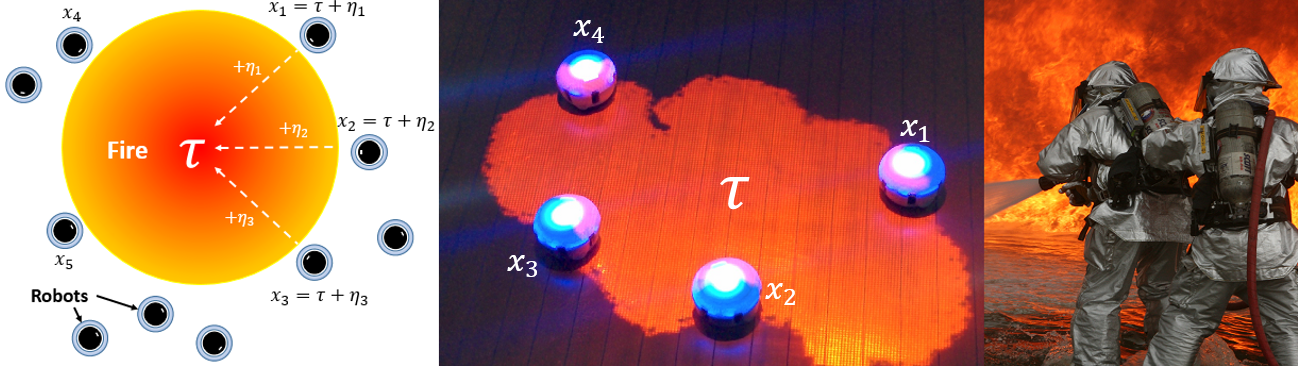
\includegraphics[width=\textwidth]{../figures/dropletfire.png}
\centering\caption{\textbf{Left:} A multi-robot firefighting scenario set up as a global game. Each player's imperfect estimate of the task is represented by $x_i$, a sum of the global magnitude parameter-$\tau$ and noisy sensor measurements-$\eta_i$. \textbf{Center:} The same scenario set up using actual robots and a projected fire, inspired from real forest fire containment (\textbf{Right}).}\label{fig:ggsetup}
\end{figure*}

\subsection{Formal Definition of a Concurrent Benefit Task}
We define a task $T$ to be a \textit{concurrent benefit task} if: 
\begin{enumerate}[a.]
	\item $u_i(a_i,g,\tau)$ is a non-decreasing and continuous function of $\tau$ for any $a_i\in A_i$ and $g$. 
	\item For extreme magnitude ranges, taking part in the activity has unique trivial equilibrium, i.e. there exists $\underline{\tau},\bar{\tau}\in (c,d)$ with $\underline{\tau}\leq \bar{\tau}$ such that for any $\tau\geq \bar{\tau}$, the only equilibrium of the game is $(1,1,\ldots,1)$ and for $\tau\leq \underline{\tau}$, the only equilibrium of the game is $(0,0,\ldots,0)$.
\end{enumerate}

Note that in order to have such a task, we need the above conditions to hold for all the robots, i.e. for all $i\in\{1,\ldots,n\}$.
An example of a utility function that would satisfy such conditions is a function $u_i(a_i,g,\tau)=a_i(1-e^{-(g+1)}+\tau)$.

The main challenge in devising strategies in performing a concurrent benefit task is that the knowledge of the magnitude parameter is not easily accessible to the robots. For example consider the firefighting scenario described above. The magnitude of the task is not easily estimated by each robot and they only have noisy, imperfect information through their on-board sensors and their local measurements.  We model this imperfect knowledge by assuming that robot $i$ observes $x_i=\tau+\eta_i$ where $\eta_i$ is a Gaussian $\mathcal{N}(0,\sigma_i^2)$ random variable, as seen in Fig.~\ref{fig:ggsetup}. Now, the main questions is that given a robot's private measurement $x_i$, what is a \textit{sensible strategy} to follow. 

To define what a \textit{sensible strategy} is, let us first define what we mean by a \textit{strategy}. We call a function that maps measurements (observations) to actions $A_i$ a strategy. Mathematically, a strategy $s_i$ for the $i$th robot is a (measurable) function $s_i:\R\to A_i$. Indeed a strategy $s_i$ prescribes what action the $i$th robot should take given its own measurement $x_i$. Now, consider a set of robots with strategies $s_1,\ldots,s_n$. Let us define the strategies of the robots, except the $i$th robot, to be the vector $s^{-i}=(s_1,\ldots,s_{i-1},s_{i+1},\ldots,s_n)$. For the $i$th robot, we define the best-response $BR(s^{-i})$ (to the strategies of the other robots) to be a strategy $\tilde{s}$ that for any $x\in \R$: 
\begin{align*}\label{eqn:BR}
BR(s^{-i})(x)&=\tilde{s}(x)=\argmax_{a_i\in A_i} E(u_i(a_i,g,\tau)\mid x_i=x)\cr 
&=\argmax_{a_i\in A_i} E(u_i(a_i,\sum_{j\not=i}s_j(x_j),\tau)\mid x_i=x)
\end{align*}
Note that given $x_i$ and the strategies of the other robots $s^{-i}=(s_1,s_2,\ldots,s_{i-1},s_{i+1},\ldots,s_n)$, $\tau$, and $s_j(x_j)$ will be a random variable. In other words, given the $i$th robot's observation $x_i$, the observation of the other robots and hence, their actions would be still random as the observations of different robots are independent. We say that a strategy $s_i$ is a threshold strategy if $s_i(x)=\text{step}(x-t_i)$ where $\text{step}(x)$ is the step function which is $1$ for $c\geq 0$ and $0$ for $c<0$.

Now, we are ready to define what we mean by a \textit{sensible strategy}. We say that a strategy profile $s=(s_1,\ldots,s_n)$ is a Bayesian Nash Equilibrium if $s_i=BR(s^{-i})$ for all $i\in \{1,\ldots,n\}$. In other words, with the current strategies of the $n$ robots, no robots has the incentive to deviate from its current strategy.

\subsection{Theorem and Proof}\label{sec:thmproof}
\begin{theorem}
Let task $T$ be a concurrent benefit task. Suppose that the magnitude parameter $\tau$ is a continuous random variable over $\R$ (or a closed and connected subset of $\R$). Also, suppose that $x_i=\tau+\eta_i$ where $\eta_1,\ldots,\eta_n$ are independent Gaussian random variables. Then, there exists a strategy profile $s=(s_1,\ldots,s_n)$ of threshold policies that is a Bayesian Nash Equilibrium.
\end{theorem}
\begin{proof}
First, we show that the best-response to a threshold strategy $s$ profile is a threshold strategy profile $\tilde{s}$. To see this, note that if for some observation $x_i=x$, $BR(s^{-i})(x)=1$, then since $u_i$ is a non-decreasing function of $\tau$ and also, the fact that all other agents are using the same strategy profile, then it follows that $BR(s^{-i})(y)=1$ for $y\geq x$. The same argument holds for an $x$ with $BR(s^{-i})(x)=0$ which implies that $BR(s^{-i})(y)=0$ for $y\leq x$. Therefore, $BR(s^{-i})$  is a threshold policy. Now, consider threshold strategies $s_1,\ldots,s_n$ with thresholds $t_1,t_2,\ldots,t_n$ and let the best response to these strategies have thresholds $\tilde{t}_1,\ldots,\tilde{t}_n$, respectively. If $t_i$ is sufficiently large, then the second property of the concurrent benefit tasks implies that the $\tilde{t}_i\leq t_i$ because large enough measurement $x_i$ implies that agent $i$ himself should take part in the task. Similarly, for sufficiently low threshold $t_i$, we will have $\tilde{t}_i\geq t_i$. Therefore, the best response function would map the set of thresholds in a big enough (convex) box to itself and hence, by the Brouwer's fix point theorem, we have that there exists a threshold strategy $s^*$ that will map to itself through the best response mapping which happens if and only if $s^*$ is a Bayesian Nash equilibrium. 
\end{proof}



\section{Discussion}\label{sec:disc}
\textbf{To be completed\ldots}



\section{Conclusion}\label{sec:conc}
\textbf{To be completed\ldots}



%%%%%%%%%%%%%%%%%%%%%%%%%%%%%%%%%%%%%%%%%%%%%%%%%%%%%%%%%%%%%%%%%%%%%%%%%%%%%%%%
%%%%%%%%%   The Bibliography, if any   %%%%%%%%%
\bibliographystyle{IEEEtran}		% or "siam", or "alpha", etc.
%\nocite{*}
\bibliography{../refworks}
\end{document}
